\documentclass[12pt, titlepage]{article}

\usepackage{float}
\usepackage{geometry}
\usepackage{booktabs}
\usepackage{tabularx}
\usepackage{hyperref}
\usepackage{siunitx}
\hypersetup{
    colorlinks,
    citecolor=blue,
    filecolor=black,
    linkcolor=red,
    urlcolor=blue
}
\usepackage[round]{natbib}
\usepackage{amsmath, mathtools}
\usepackage{xr}


\input{../Comments}
%% Common Parts

\newcommand{\progname}{Baja Dynamics} % PUT YOUR PROGRAM NAME HERE
\newcommand{\authname}{Team \#17, Team Name
\\ Grace McKenna
\\ Travis Wing
\\ Cameron Dunn
\\ Kai Arseneau} % AUTHOR NAMES                  

\usepackage{hyperref}
    \hypersetup{colorlinks=true, linkcolor=blue, citecolor=blue, filecolor=blue,
                urlcolor=blue, unicode=false}
    \urlstyle{same}
                                


\newcommand{\refdata}[2]{
  \href{https://github.com/gr812b/CVT-Simulator/blob/main/experimental-data/#1
  }{\texttt{#2}}}


\begin{document}

\title{Usability Report for \progname{}} 
\author{\authname}
\date{\today}
	
\maketitle

\pagenumbering{roman}

\section*{Revision History}

\begin{tabularx}{\textwidth}{p{3cm}p{2cm}X}
\toprule {\bf Date} & {\bf Version} & {\bf Notes}\\
\hline
April 4th & 1.0 & Initial Version\\
\midrule

\bottomrule
\end{tabularx}

~\\

\newpage

\tableofcontents



\newpage


\newpage

\pagenumbering{arabic}

\section{Introduction}

The purpose of this document is to evaluate the usability and understandability of the CVT simulator system. The method used to evaluate user feedback was a feedback survey that included Likert-scale questions and open-ended responses.
The survey can be found \href{https://forms.office.com/r/RkeDW31ZTS}{here}. 
The survey was completed by six McMaster Baja Team members.

\section{Usability of the System}

\subsection{Format of Usability Tests}

The below test are to verify the usability of the system.
They are based on NFR2 from the \href{https://github.com/gr812b/CVT-Simulator/blob/main/docs/SRS/SRS.pdf}{SRS document}.

\begin{enumerate}

  \item \label{usetest-1}test-1\\

Type: Manual
					
Initial State: 
					
Input/Condition: Users within the Primary User role as well as Baja team members are asked to rate how simple the navigation process of the main interface. 
They are asked to rate this on a scale of (1-5) 1 being extremely difficult and 5 being extremely easy with the other options being 4: somewhat easy, 3: neutral and 2: somewhat difficult. 
					
Output/Result: The average output rating from all users is greater than or equal to a 4(somewhat easy or above expectations).
					
How test will be performed: Each user in the test group will be provided with a survey which provides a series of questions and a scale for each option where 1 represents Poor, 2 represents below expectation, 3 represents satisfactory, 4 represents above average and 5 represents excellent.
The average rating will then be calculated and must be above or equal to 4 representing the system usability is above expectations.  

\item \label{usetest-2}test-2\\

  
Type: Manual
            
Initial State: The user has successfully installed the system on their device.
            
Input/Condition: Users within the Primary User role as well as Baja team members are asked to rate the features inputting parameters, adjusting parameters, viewing data outputs and saving and exporting data on how easy it was to use each feature.
They are asked to rate this on a scale of (1-5) 1 being extremely difficult and 5 being extremely easy with the other options being 4: somewhat easy, 3: neutral and 2: somewhat difficult. 
            
Output/Result: The average output rating from all users for each listed feature is greater than or equal to a 4(somewhat easy or above expectations).
            
How test will be performed: Each user in the test group will be provided with a survey which provides a series of questions and a scale for each option where 1 represents Poor, 2 represents below expectation, 3 represents satisfactory, 4 represents above average and 5 represents excellent.
The average rating will then be calculated and must be above or equal to 4 representing the system usability is above expectations. 
  
\end{enumerate}

\subsection{Results of Usability Tests}

\begin{enumerate}
  \item test-\ref{usetest-1}
  \begin{figure}[H] 
    \centering
    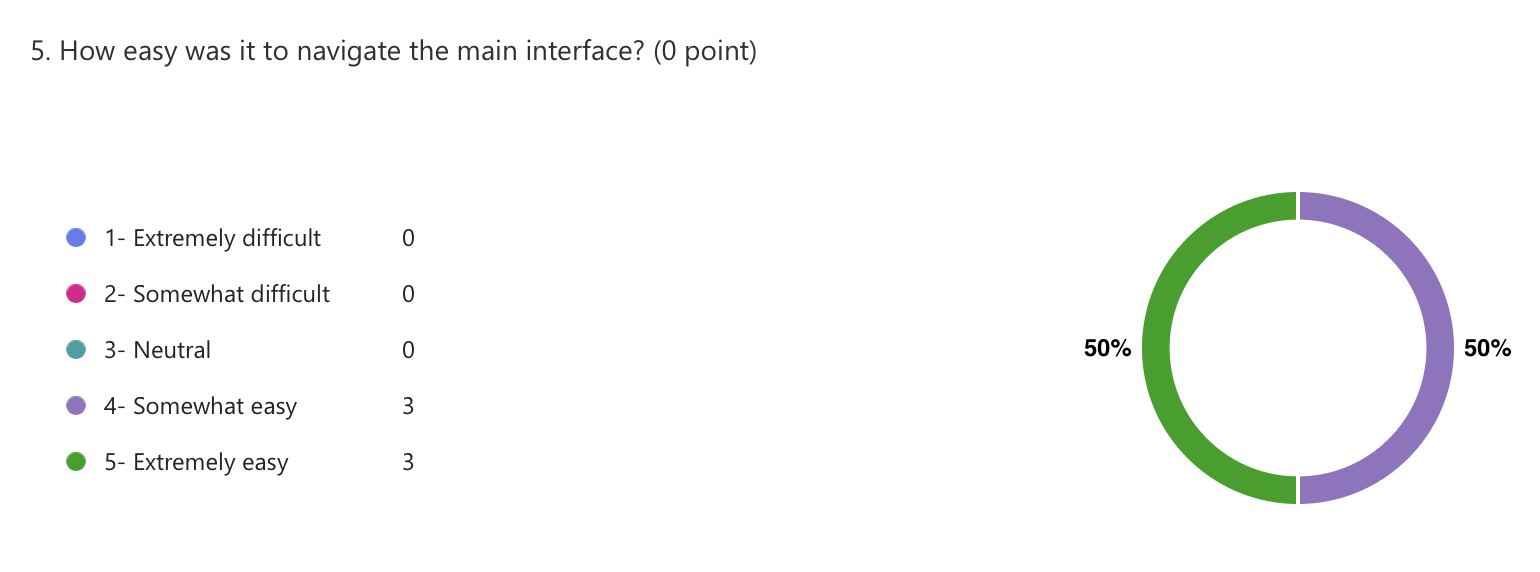
\includegraphics[width=0.9\textwidth]{use-test1.png} 
    \caption{Results from Usability test-1.}
    \label{fig:myimage}
  \end{figure}
  The average score usability test-\ref{usetest-1} is 4.5.
  \item test-\ref{usetest-2}
  \begin{figure}[H] 
    \centering
    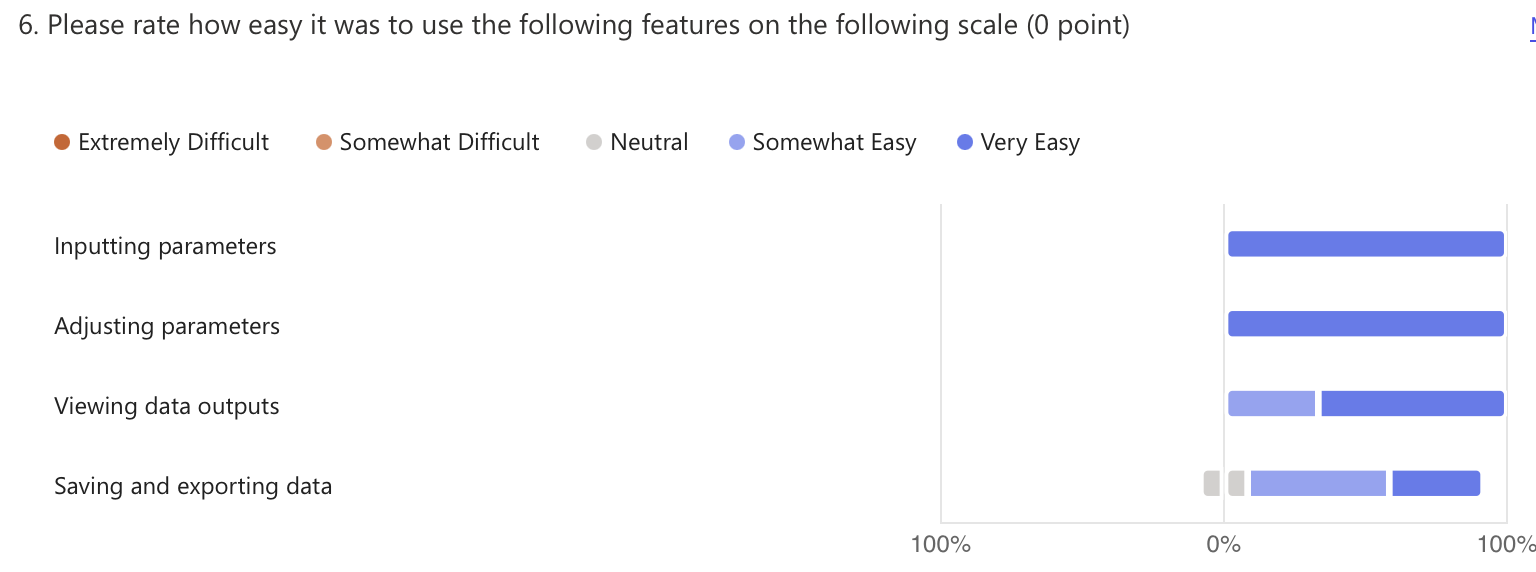
\includegraphics[width=0.9\textwidth]{use-test2.png}  
    \caption{Results from Usability test-2.}
    \label{fig:myimage}
  \end{figure}
  The average score for inputting parameters and adjusting parameters is a 5. The average score for viewing data outputs is 4.67. 
  The average score for saving and exporting data is 4.16.
\end{enumerate}

\subsection{Summary of Usability Test Results}
All average scores across both usability tests were above 4, demonstrating that users found the system intuitive and easy to interact with. 
These results indicate that the simulator meets the usability criteria, successfully passing both usability tests.

\section{Understandability of the System}

\subsection{Format of Understandability Tests}

The below test are to verify the understandability of the system.
They are based on NFR2 from the \href{https://github.com/gr812b/CVT-Simulator/blob/main/docs/SRS/SRS.pdf}{SRS document}.

\begin{enumerate}

  \item \label{undtest-1}test-1\\

  
  Type: Manual.
            
  Initial State: The user has successfully installed the system on their device.
            
  Input/Condition: Users within the Primary User role as well as Baja team members are asked to rate how clear they found the features and functions within the system. 
  They are asked to rate this on a scale of (1-5) 1 being extremely unclear and 5 being extremely clear with the other options being 4: somewhat clear, 3: neutral and 2: somewhat unclear. 
            
  Output/Result: The average output rating from all users for each listed feature is greater than or equal to a 4(somewhat clear or above expectations).
            
  How test will be performed: Each user in the test group will be provided with a survey which provides a series of questions and a scale for each option where 1 represents Poor, 2 represents below expectation, 3 represents satisfactory, 4 represents above average and 5 represents excellent.
  The average rating will then be calculated and must be above or equal to 4, representing the systems understandability is above expectations.  
  
  \item \label{undtest-2}test-2\\

  
  Type: Manual
            
  Initial State: The user has successfully installed the system on their device.
            
  Input/Condition: Users within the Primary User role as well as Baja team members are asked to rate their understanding of the simulation results and outputs. 
  They are asked to rate this on a scale of (1-5) 1 being extremely unclear and 5 being extremely clear with the other options being 4: somewhat clear, 3: neutral and 2: somewhat unclear. 
            
  Output/Result: The average output rating from all users for each listed feature is greater than or equal to a 4(somewhat clear or above expectations).
            
  How test will be performed: Each user in the test group will be provided with a survey which provides a series of questions and a scale for each option where 1 represents Poor, 2 represents below expectation, 3 represents satisfactory, 4 represents above average and 5 represents excellent.
  The average rating will then be calculated and must be above or equal to 4, representing the systems' understandability is above expectations. 
  
  \end{enumerate}

  \subsection{Results of Understandability Tests}

  \begin{enumerate}
    \item test-\ref{undtest-1}
    \begin{figure}[H]  % h = here; other options: t=top, b=bottom, p=page of floats
      \centering
      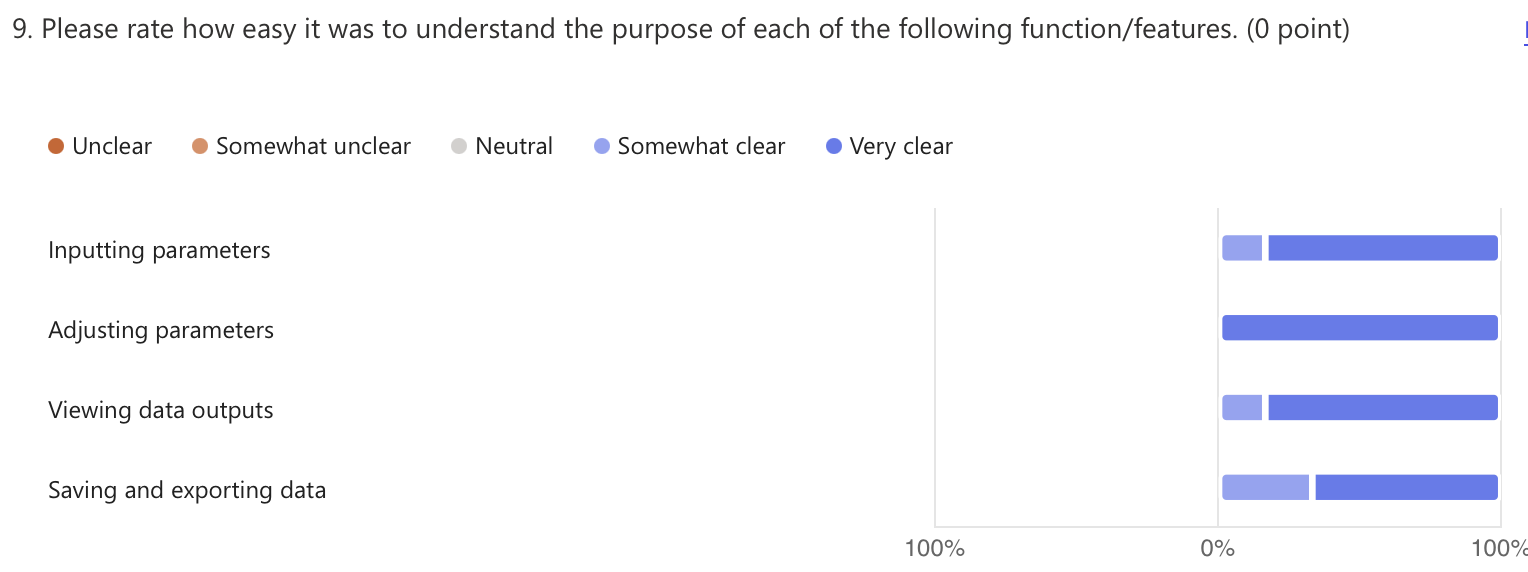
\includegraphics[width=0.9\textwidth]{und_test1.png}  % Adjust width as needed
      \caption{Results from Understandability test-1.}
      \label{fig:myimage}
    \end{figure}
    The average score for inputting parameters is 4.83, the average score for adjusting parameters is 5. The average score for viewing data outputs is 4.83 and the average score for saving and exporting data is 4.67.
    \item test-\ref{undtest-2}
    \begin{figure}[H]  % h = here; other options: t=top, b=bottom, p=page of floats
      \centering
      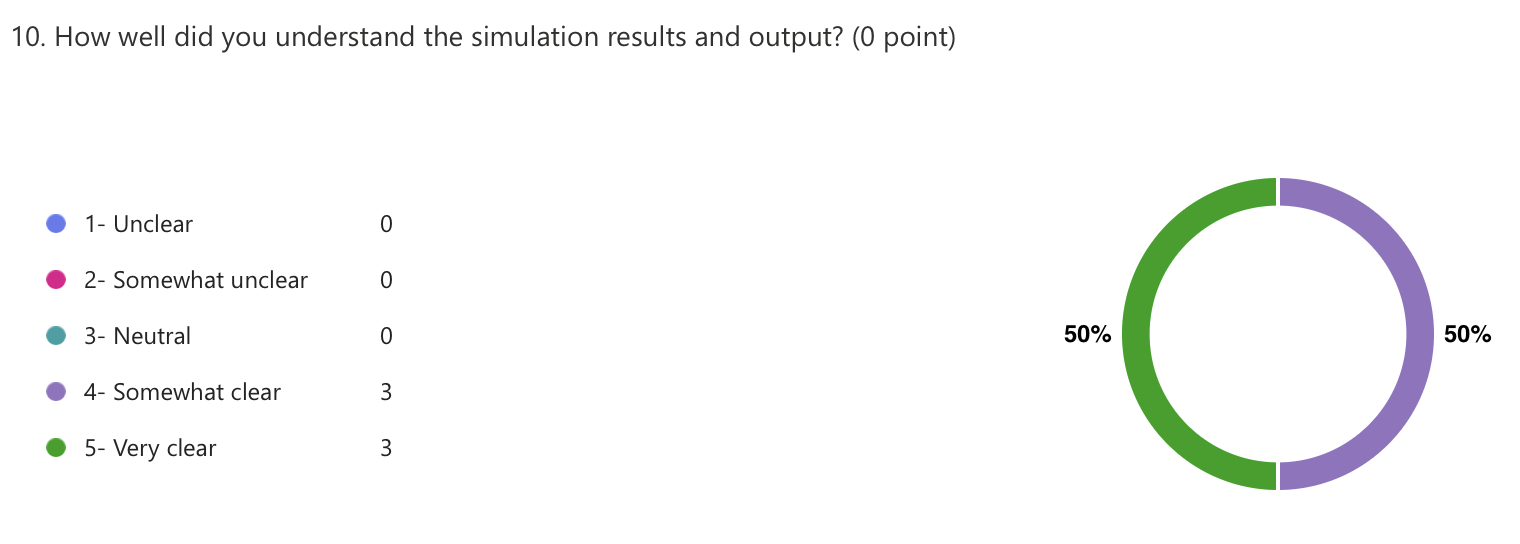
\includegraphics[width=0.9\textwidth]{und_test2.png}  % Adjust width as needed
      \caption{Results from Understandability test-2.}
      \label{fig:myimage}
    \end{figure}
    The average score for understandability test-\ref{undtest-2} is 4.5.
  \end{enumerate}

  \subsection{Summary of Understandability Test Results}
  All average scores across both understandability tests were above 4, indicating that users were able to comprehend the purpose of each function and interpret the simulation results effectively. These findings suggest that the simulator meets the criteria for understandability and successfully supports user interpretation and decision-making.

  \section{Overall Satisfaction and Feedback}
  \subsection{Results of Overall Satisfaction and Feedback}
  \begin{enumerate}
    \item Overall Satisfaction
    \begin{figure}[H]  % h = here; other options: t=top, b=bottom, p=page of floats
      \centering
      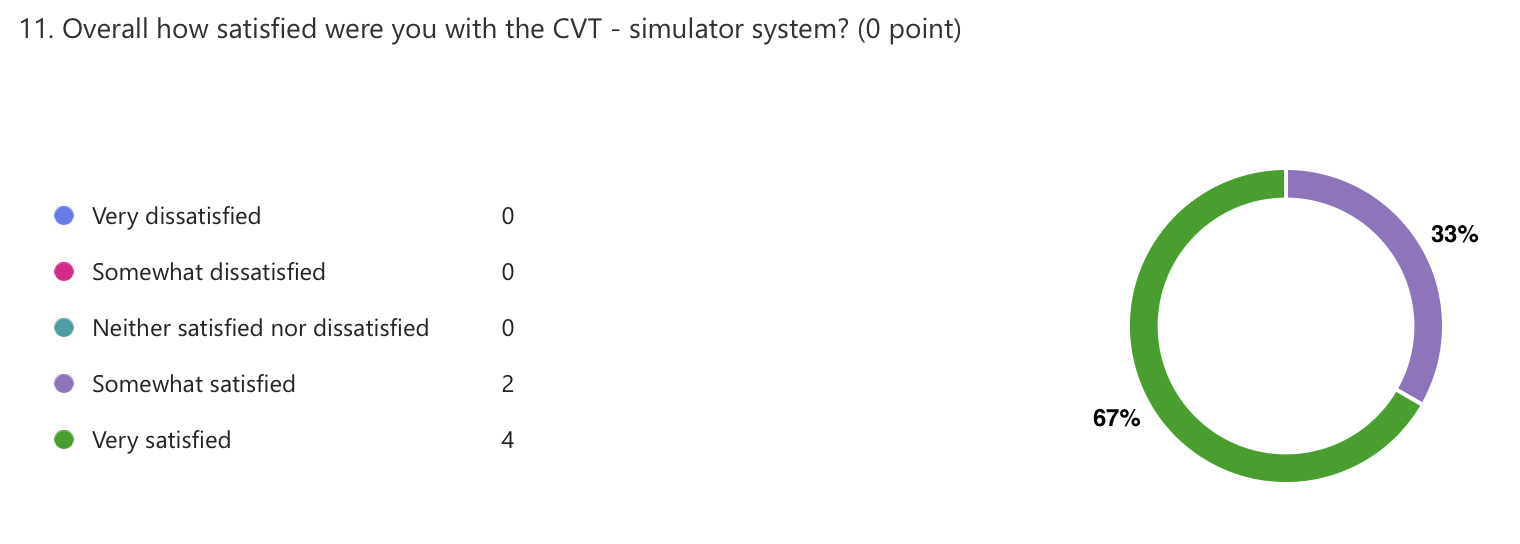
\includegraphics[width=0.9\textwidth]{overall.png}  % Adjust width as needed
      \caption{Results from Understandability test-2.}
      \label{fig:myimage}
    \end{figure}
    The average score for this question was 4.67.
  \end{enumerate}

\subsection{Summary of Understandability Test Results}

Overall, users responded positively to the system, indicating that they found it both usable and understandable. 
The feedback suggests that the simulator effectively supports user interaction, contributing to a generally satisfying user experience.
\section{Recommendations}

One limitation of this evaluation is that only six participants completed the survey, which provides a limited sample size. 
Given more time, we would have aimed to gather feedback from a larger group of users to strengthen the reliability of the findings.
\section{Conclusion}

The usability and understandability evaluations of the CVT simulator indicate that users generally found the system intuitive, functional, and easy to interpret. 
While the limited number of survey responses restricts the breadth of insights, the overall positive feedback suggests that the simulator is well-designed and effective in supporting user interaction. 
Future testing with a larger user base would provide additional validation and help guide further refinements.

\newpage{}




\end{document}